%%%%%
%%
%% Chalmers University of Technology Master's Thesis Template
%%
%% Jonas Einarsson (2010)
%% Adapted from work by Joel Goop
%%
%% Uses references.bib as Bibtex source
%% Uses elsevier numerical style .bst (change in settings.tex)
%%
%% DON'T FORGET: Change PDF metadata in settings.tex !!
%%
%%%%%
\documentclass[11pt,a4paper,twoside,openleft]{report}

% Packages and commands file
\usepackage[utf8]{inputenc}
\usepackage[T1]{fontenc}
\usepackage[english]{babel}
\usepackage{amsmath}
\usepackage{amsthm}
\usepackage{ae}
\usepackage{icomma}
\usepackage{units}
\usepackage{color}
\usepackage{graphicx}
\usepackage{epstopdf}
\usepackage{subfigure}
\usepackage{bbm}
\usepackage{caption}
\usepackage[square, numbers, sort]{natbib}
\usepackage{multirow}
\usepackage{array}
\usepackage{geometry}
\usepackage{fancyhdr}
\usepackage{fncychap}
\usepackage[hyphens]{url}
\usepackage[breaklinks,pdfpagelabels=false]{hyperref}
\usepackage{lettrine}
\usepackage{eso-pic}
\usepackage{datetime}
\usepackage{natbib}
\usepackage{cleveref}
\usepackage{listings}
\usepackage{tikz}

\usetikzlibrary{arrows,automata,positioning,shadows}

% \newState{}{}{}{}
%
% #1: internal name,
% #2: (visible) label,
% #3: node properties (e.g. accepting, initial)
% #4: relative position (e.g. right of=/left of=/above of=/below of=)

\newcommand{\newState}[4]{\node[state,#3](#1)[#4]{#2};}

% \newTransition{}{}{}{}
% #1: source state (internal name),
% #2: target state (internal name)
% #3: guard/edge label
% #4: edge direction (loop below/above, bend right/left)
\newcommand{\newTransition}[4]{\path[->] (#1) edge [#4] node {#3} (#2); } 


\newcommand{\rd}{\ensuremath{\mathrm{d}}}
\newcommand{\id}{\ensuremath{\,\rd}}
\newcommand{\degC}{\ensuremath{\,\unit{^\circ C}}}

% Fancyheader shortcuts
\newcommand{\setdefaulthdr}{%
\fancyhead[L]{\slshape \rightmark}%
\fancyhead[R]{\slshape \leftmark}%
\fancyfoot[C]{\thepage}%
}
\newcommand{\setspecialhdr}{%
\fancyhead[L]{ }%
\fancyhead[R]{\slshape \leftmark}%
\fancyfoot[C]{\thepage}%
}

\newcommand{\mail}[1]{\href{mailto:#1}{\nolinkurl{#1}}}
\newcommand{\backgroundpic}[3]{%
	\put(#1,#2){
		\parbox[b][\paperheight]{\paperwidth}{%
			\centering
			\includegraphics[width=\paperwidth,height=\paperheight,keepaspectratio]{#3}
			\vfill
}}}
\newtheorem{theorem}{Theorem}[section]
\newtheorem{corollary}[theorem]{Corollary}
\newtheorem{lemma}[theorem]{Lemma}

\theoremstyle{remark}
\newtheorem{remark}[theorem]{Remark}

\theoremstyle{definition}
\newtheorem{definition}[theorem]{Definition}
\theoremstyle{definition}
\newtheorem{example}[theorem]{Example}



% Settings (Metadata)
% References, choose bst-file
\bibliographystyle{elsart-num}

% DateFormat
\newdateformat{mydate}{\monthname[\THEMONTH] \THEYEAR}

% PDF Metadata and link styles
\hypersetup{
		pdftitle={Master's Thesis: },%
		pdfauthor={Jonas Einarsson},%
    colorlinks=true,%
    citecolor=black,%
    filecolor=black,%
    linkcolor=black,%
    urlcolor=black
}


% Dropping initial letter color
\renewcommand{\LettrineFontHook}{\color[gray]{0.5}}

% Chapter headings style (fncychap)
\makeatletter
\ChNumVar{} % sets the style for digit
\ChTitleVar{\Huge\bfseries\centering} % sets the style for title
\ChRuleWidth{4pt} % Set RW=4pt
\ChNameUpperCase % Make name uppercase
\renewcommand{\DOCH}{
\centering
{\CNoV {\fontsize{60pt}{20pt}\selectfont\thechapter} }
\vskip 40\p@}
\renewcommand{\DOTI}[1]{%
\CTV\FmTi{#1}\par\nobreak
\vskip 40\p@}
\renewcommand{\DOTIS}[1]{%
\CTV\FmTi{#1}\par\nobreak
\vskip 40\p@}
\makeatother

% Single page abstract
\renewenvironment{abstract}%
{\begin{center} \bfseries \abstractname \end{center}}%
{\vspace{2\baselineskip}}%

% Figure & Table captions
\captionsetup{margin=10pt,font=small,labelfont=bf}
\captionsetup[table]{position=top}
\setlength{\extrarowheight}{4pt}
\addtolength{\headheight}{\baselineskip}

% Fancyheader (see packagescommands.tex for default/special)
\pagestyle{fancy}
\setspecialhdr

% Stolen settings (unknown origin):
% Alter some LaTeX defaults for better treatment of figures:
% See p.105 of "TeX Unbound" for suggested values.
% See pp. 199-200 of Lamport's "LaTeX" book for details.
%   General parameters, for ALL pages:
\renewcommand{\topfraction}{0.9}	% max fraction of floats at top
\renewcommand{\bottomfraction}{0.8}	% max fraction of floats at bottom
%   Parameters for TEXT pages (not float pages):
\setcounter{topnumber}{2}
\setcounter{bottomnumber}{2}
\setcounter{totalnumber}{4}     % 2 may work better
\setcounter{dbltopnumber}{2}    % for 2-column pages
\renewcommand{\dbltopfraction}{0.9}	% fit big float above 2-col. text
\renewcommand{\textfraction}{0.07}	% allow minimal text w. figs
%   Parameters for FLOAT pages (not text pages):
\renewcommand{\floatpagefraction}{0.7}	% require fuller float pages
% N.B.: floatpagefraction MUST be less than topfraction !!
\renewcommand{\dblfloatpagefraction}{0.7}	% require fuller float pages

% remember to use [htp] or [htpb] for placement


\begin{document}

% Title page and abstract
% Chalmers title page
\begin{titlepage}
\AddToShipoutPicture{\backgroundpic{-4}{56.7}{fig/auxiliary/frontpage}}
\mbox{}
\vfill
\addtolength{\voffset}{2cm}
\begin{flushleft}
	{\noindent {\Huge A Generator of Divide-and-Conquer
Lexers} \\[0.5cm]
	\huge A Tool to Generate an Incremental Lexer from a Lexical Specification \\[0.5cm]
	\emph{\Large Master of Science Thesis [in the Programme MPALG]} \\[.8cm]
	
	{\huge JONAS HUGO}\\[.8cm]
	{\huge KRISTOFER HANSSON}\\[.8cm]
	
    {\Large
	\textsc{Chalmers University of Technology} \\
	Department of Computer Science and Engineering \\
	Göteborg, Sweden,  \mydate\today\\
	} 
	}
\end{flushleft}

\newpage

\ClearShipoutPicture
\pagestyle{empty}
\begin{flushleft}
    {\noindent{
The Author grants to Chalmers University of Technology and University of       Gothenburg  the non-exclusive right to publish the Work electronically and in a non-commercial purpose make it accessible on the Internet. 
The Author warrants that he/she is the author to the Work, and warrants that the Work does not contain text, pictures or other material that violates copyright law. \\[0.5cm]


The Author shall, when transferring the rights of the Work to a third party (for example a publisher or a company), acknowledge the third party about this agreement. If the Author has signed a copyright agreement with a third party regarding the Work, the Author warrants hereby that he/she has obtained any necessary permission from this third party to let Chalmers University of Technology and University of Gothenburg  store the Work electronically and make it accessible on the Internet.\\[2cm]

An not to long headline describing the content of the report \\
A Subtitle that can be Very Much Longer if Necessary\\

JONAS HUGO, \\
KRISTOFER HANSSON, \\[0.8cm]

© JONAS HUGO, \mydate\today.\\
© KRISTOFER HANSSON, \mydate\today.\\[0.5cm]

Examiner: NAME A. FAMILYNAME\\[0.5cm]

Chalmers University of Technology\\
University of Gothenburg\\
Department of Computer Science and Engineering\\
SE-412 96 Göteborg\\
Sweden\\
Telephone + 46 (0)31-772 1000\\[0.8cm]

Cover:\\
an explanatory caption for the (possible) cover picture\\
with page reference to detailed information in this essay.\\[0.5cm]

Department of Computer Science and Engineering\\
Göteborg, Sweden \mydate\today

    }
    }

\end{flushleft}

\end{titlepage}
% End Chalmers title page

\pagestyle{empty}
\newpage
\clearpage
\mbox{}
\newpage
\clearpage
\thispagestyle{empty}

\begin{abstract}
Lorem ipsum dolor sit amet, consectetur adipisicing elit, sed do eiusmod tempor incididunt ut labore et dolore magna aliqua. Ut enim ad minim veniam, quis nostrud exercitation ullamco laboris nisi ut aliquip ex ea commodo consequat. Duis aute irure dolor in reprehenderit in voluptate velit esse cillum dolore eu fugiat nulla pariatur. Excepteur sint occaecat cupidatat non proident, sunt in culpa qui officia deserunt mollit anim id est laborum.
\end{abstract}

\newpage
\clearpage
\mbox{}
\newpage
\clearpage
\thispagestyle{empty}
\section*{Acknowledgements}
Lorem ipsum dolor sit amet, consectetur adipisicing elit, sed do eiusmod tempor incididunt ut labore et dolore magna aliqua. Ut enim ad minim veniam, quis nostrud exercitation ullamco laboris nisi ut aliquip ex ea commodo consequat. Duis aute irure dolor in reprehenderit in voluptate velit esse cillum dolore eu fugiat nulla pariatur. Excepteur sint occaecat cupidatat non proident, sunt in culpa qui officia deserunt mollit anim id est laborum. \\[1cm]

\hfill The Authors, Location 11/9/11
\newpage
\clearpage
\mbox{}


% Table of contents
\newpage
\pagenumbering{roman}
\setcounter{page}{1}
\pagestyle{fancy}
\setspecialhdr
\tableofcontents

% Main area
\newpage
%\setdefaulthdr
\fancyhead{}
\fancyhead[LE]{\leftmark}
\fancyhead[RO]{\rightmark}
\pagenumbering{arabic}	
\setcounter{page}{1}
% Content
\chapter{Introduction}
Editors normally have regular-expression based parsers, which are efficient and
robust, but lack in precision: they are unable to recognize complex structures.
Parsers used in compilers are precise, but typically not robust: they fail to
recover after an error. They are also not efficient for editing purposes,
because they have to parse files from the beginning, even if the user makes
incremental changes to the input. More modern IDEs use compiler strength
parsers, but they give delayed feedback to the user. Building a parser with good
characteristics is challenging: no system offers such a combination of
properties.

In order to implement a parser with the characteristics described above; robust,
precise and efficient; a lexer that has the same properties is needed. This
project aims to implement such a lexer.

\section{Scope of work}
Existing lexical analyzers are sequential. When the text is updated the lexer
must start the lexical analysis from the beginning. The goal of this project is
to create an algorithm that, after an update to the text, only needs to
recalculate the updated and the part of the result effected by the update. The
recalculation should have time complexity $\theta log(n)$ in order to be run in
real time, for example in a text editor with immediate update.

The report gives a general understanding of how lexical analyzers work and what
tools are needed for a divide and conquer implementation to work. An overview of
the ideas behind a divide and conquer lexer is explained in order to give enough
understanding for the algorithm this report purposes. A robust implementation of
the algorithm is presented with explanations on how different cases are handled.
Tests for preciseness, time performance and space performance are explained and
their corresponding result are presented. The report will present a discussion
on where a divide and conquer lexer is useful.

\section{Related Work}
This project revolves around the idea of using incremental regular expressions.
Piponi \cite{blog} wrote a blog post about how to implement incremental regular
expressions using finger trees. The solution to matching regular expressions
incrementally in the blog post gives a good starting point to this project,
however a lexer do not match a string against one expression. A lexer matches a
string against a set of regular expressions and returns which expressions where
matched and in what order rather then answering if the string matched the
expressions \cite{blog}.

Bernardy and Claessen \cite{bernardyefficient2013} wrote a paper titled 
``Efficient Divide-and-Conquer Parsing of Practical Context-Free Languages''
that describes and efficient parallel parser built on Valiants algorithm
\cite{valiantgeneral1975}. The paper proves that for a defined set of input
the complexity for the parser will be $\theta log^3(n)$.
Since the implementation of the parser is done in BNFC \cite{bnfc} it uses a
sequential lexer generated by alex \cite{alex}. The lexical analyzer this
project purposes is a divide and conquer solution which could be integrated to
the parser purposed by Bernardy and Claessen to get a divide and conquer
solution from the programming code to the result of the parser.

\chapter{Lexer}
A Lexer, lexical analyser, is a pattern matcher. It's job is to find sequence 
of characters in a larger string. The Lexer is a front end of a syntax 
analyser. \cite{sebesta2012}
This can be done by using regular expressions, regular sets and finite
automata. Which are central concepts in formal language theory. \cite{Aho1990}
All on which will be described in this chapter.

\section{Lexing vs Parsing}
There are several reasons why a compiler should be separated in to lexical 
analyser and a parser (syntax analyser) phases. Simplicity of design is the most
important reason. When dividing the task in to these to sub task, it allows the
system to simplify one of these sub-tasks. For example, a parser that has to 
deal with white-spaces and comments as syntactical units would be more complex 
then one that can assume white-spaces and comments have already been removed by 
an lexer. Also when the two tasks are divided into sub-tasks it can lead to 
cleaner overall design when designing a new language \cite{Aho2006}
Lexers work as a subprogram to the parser, giving it's result to the syntax 
analyser. So the only thing the syntax analyser will see is the output from the 
lexer, tokens and lexemes which will be described later in this chapter. 
\cite{sebesta2012}
The lexer also skips comments and white-spaces, since these are not relevant 
for the syntax analyser. \cite{sebesta2012}
Also overall efficiency of the compiler can be improved. When separating the 
lexical analyser it allows for appliance of specialised techniques that serve 
only the lexical task. \cite{Aho2006}
Last compiler portability can be enhanced. That is Input-device-specific 
peculiarities can be restricted to the lexical analysis. \cite{Aho2006}
So the lexer can detect syntactical errors in tokens, such as ill-formed 
floating-points literals, and report these errors to the user. 
\cite{sebesta2012} Breaking the compilation before running the syntax analyser, 
saving computing time. 
\section{Token Specification}
A lexical analyser job is to translate a human readable string to a abstract 
computer readable list of tokens. To define these abstract data-types in form of
strings the lexer uses different techniques. This section will describe these
techniques used when writing rules for the tokens patterns. 
\subsection{Languages}
An alphabet is an finite set of symbols, such an alphabet is for example the 
Unicode, which includes approximately $100,000$ characters. A language is any 
countable set of strings over some fixed alphabet. \cite{Aho2006}
The term formal languages refers to languages which can be described by a body 
of systematic rules. Like any formal language, a regular language is a set of 
strings. In other words a sequence of symbols, from a finite set of symbols. 
Only some formal languages are regular; in fact, regular languages are exactly 
those that can be defined by regular expressions. \cite{Ranta2012}
\subsection{Regular Expressions}
Say that we want to express the set of valid C identifiers. Use of regular 
expressions make it very easy, as shown in \cref{regexpEx}. 
\begin{example}[Valid C Idents]\label{regexpEx} \cite{Aho2006}\\
Say we have a element $letter \in \{$a$ \dots $z$\} \cup \{$A$ \dots $Z$\} \cup 
\{$\_$\}$
and another element $digit \in \{0 \dots 9\}$
Then with help of regular expressions the definition of all valid C identifiers 
would look like this: $letter (letter | digit)*$. 
\end{example}
In \cref{regexp} is the formal definition for regular expressions.
\begin{definition}[Regular Expressions]\label{regexp} \cite{Aho1990}
\begin{enumerate}
  \item The following characters are meta characters $\{ '|', '(', ')', '*' \}$.
  \item A none meta character $a$ is a regular expression that matches the 
      string $a$.
  \item If $r_1$ and $r_2$ are regular expressions then $(r_1 | r_2)$ is a 
      regular expression that matches any string that matches $r_1$ or $r_2$.
  \item If $r_1$ and $r_2$ are regular expressions. $(r_1)(r_2)$ is a regular
      expression of the form that matches the string $xy$ iff $x$ matches $r_1$
      and $y$ matches $r_2$.
  \item If $r$ is a regular expression the $r*$ is a regular expression that
      matches any string of the form $x_1, x_2, \dots , x_n, n \geq 0$.
      Where $r$ matches $x_i$ for $1 \leq i \leq n$, in particular $(r)*$ 
      matches the empty string, $\varepsilon$.
  \item If $r$ is a regular expression, then $(r)$ is a regular expression that
      matches the same string as $r$.
\end{enumerate}
\end{definition}
Many parentheses can be reduced by adopting the convention that the Kleene
closure operator $*$ has the highest precedence, then concat and then or
operator $|$. The two binary operators, cancat and $|$ are left 
left-associative. \cite{Aho1990}
\subsection{Regular Definitions}
In a definition of a language it is useful to give regular expressions names, 
so they can for example be used in other regular expressions, as these names 
where themself symbols. If $\Sigma$ is an alphabet of basic symbols, then a 
regular definition is a sequence of definitions of the form:
\begin{center}
\begin{tabular}{l c r}
$d_1$ & $\to$ & $r_1$\\
$d_2$ & $\to$ & $r_2$\\
$\vdots$ & $\to$ & $\vdots$\\
$d_n$ & $\to$ & $r_n$\\

\end{tabular}
\end{center}
where:
\begin{enumerate}
\item Each $d_i$ is a new symbol, not in $\Sigma$ and not the same as any other 
of the $d$'s.
\item Each $r_i$ is a regular expression over the alphabet $\Sigma  \cup \{d_1, 
d_2 \dots d_{i-1}\}$
\end{enumerate}
By restricting $r_i$ to $\Sigma$ and previously defined $d$'s the regular 
definitions avoid recursive definitions.  
\cite{Aho2006}

\section{Tokens, Patterns and Lexemes}
When the rules are defined, the lexer needs structures of representing theses 
rules and the result from lexing the code-string. This section will describe the 
data-structures the lexical analyser works with for representing the abstract 
data. What the lexer use them for and what is sent forward to the syntactical 
analyser. 

A lexical analyser uses three different terms. All which is described here 
below. 
\begin{description}
  \item[Token]
    is a pair consisting of a token name and an optional attribute value. The 
token name is a abstract symbol corresponding to a lexical unit \cite{Aho2006}. 
For example, a particular keyword, data-type or identifier.  The token names is 
what is given to the parser. 
  \item[Pattern]
    is a description of what form a lexemes of a token may take. \cite{Aho2006} 
For example, a keyword is just the sequence of characters that forms the 
keyword, an int is just a sequence consisting of just numbers. 
  \item[Lexemes]
    is a sequence of characters in the code that is being analysed which 
matches the pattern for a token and is identified by the lexical analyser as an 
instance of a token. \cite{Aho2006}
\end{description}
As mention before a token consist of token name and a optional attribute value. 
This attribute is used when one lexeme can match more then one pattern. \cite
{Aho2006} For example the pattern for a digit token matches both $0$ and $1$, 
but it is important for the code generator to know which lexeme was found. 
Therefore the lexer often return not just the token but also an attribute value 
that describes the lexeme found in the source program corresponding to this 
token. \cite{Aho2006} A lexer collects chars into logical groups and assign 
internal codes to these groups. according to there structure.\cite{sebesta2012} 
Where the groups of chars are lexemes and the internal codes are tokens. Here 
follows a example how a small piece of code would be divided.
\begin{example}[Logical grouping] \label{codeToToken} \cite{sebesta2012} \\
This is the code being lexed:
\lstinputlisting[language=c]{examples/token.c}
This is how it will be divided:
\begin{center}
\begin{tabular}{l c}
\underline{Token} & \underline{Lexeme}\\
IDENT & result\\
ASSING\_OP & $=$\\
IDENT & oldsum\\
SUB\_OP & $-$\\
IDENT & value\\
DIV\_OP & $/$\\
INT\_LIT & 100\\
SEMICOLON & ;
\end{tabular}
\end{center}
\end{example}

\section{Recognition of Tokens}
In previous section the topic have been, how to represent a pattern using 
regular expressions and how these expressions relates to tokens. This section 
will highlight how to transform a sequence of characters into a sequence of 
abstract tokens. First some basic understanding with transition diagrams.  
\subsection{Transition Diagrams}
A state transition diagram, or just transition diagram is a directed graph. 
Where the nodes are labelled with the state name. Each node 
represent a state which could occur during the process of scanning the input 
looking for lexeme that matches one of several patterns.\cite{Aho2006} The 
edges are labelled with the input characters that causes the transition among 
the states. An edge may also contain actions the lexer must perform when 
transition is token.\cite{sebesta2012} Here follows some properties for a 
transition diagram, One state is said to be initial state. The transition 
diagram always begins at this state, before any input symbols have been read. 
Some states are said to be accepting (final). They indicate that a lexeme has 
been found. The found token should then be returned with any additional 
optional values, mentioned in previous section.\cite{Aho2006}
Transition diagrams of the formed used in lexers are representations of a class 
of mathematical machines called finite automata. Finite automata can be 
designed to recognise members of a class of languages called regular languages, 
mentioned above.
\cite{sebesta2012} 
\subsection{Finite Automata}
A finite automata are essentially graphs, like transitions diagrams, with some 
differences:
\begin{itemize}
  \item Finite automata are recognizers; they simply say "YES" or "NO" about 
each possible input string.
  \item Finite automata comes in to different forms:
    \begin{description}
      \item [Non-deterministic Finite Automata (NFA)] which have no restriction 
of the edges, several edges can be labelled by the same symbol out from the 
same state. $\epsilon$, the empty string, is a possible label. 
      \item [Deterministic Finite Automata (DFA)] for each state and for each 
symbol of its input alphabet exactly one edge with that symbol leaving that 
state
    \end{description}
\end{itemize}
Both these forms of finite automate are capable of recognising the same 
language, called regular languages. These are languages that regular 
expressions can describe. \cite{Aho2006}
The formal definition of a finite automata follows:
\begin{definition}[Finite Automata] \label{finiteAutomataDef} 
\cite{sipser2006} \\
A finite automata is a 5-tuple $(Q, \Sigma, \delta, q_0, F)$, where
\begin{enumerate}
  \item $Q$ is a finite set called the states,
  \item $\Sigma$ is a finite set called alphabet,
  \item $\delta: Q \times \Sigma \to Q$ is a transition function,
  \item $q_0 \in Q$ is the start state, and
  \item $F \subseteq Q$ is the set of accept states.
\end{enumerate}

\end{definition}
\subsubsection{Non-deterministic Finite Automata}
An NFA accept input $x$ if and only if there is a path in the transition 
diagram from the start state to one of the accepting states. Such that the 
symbols along the way spells out $x$. \cite{Aho2006}

There are two different ways of representing an NFA which this report will
describe. One is by transition diagrams, where the regular expression will be
represented by a graph structure. Another is by transitions table, where the 
regular expression will be converted in to a table of states and the 
transitions for these states given the input. The following examples shows how 
the transition diagram and transition table representation will look like for a 
given regular expression.

\begin{example}[RegExp to Transition Diagram] \label{regexp2td}
\cite{Aho2006}\\
Given this regular expression: $(a | b)* abb$ \\
the transition diagram in \cref{fig:td} representing this regular expression.
\end{example}
\begin{figure}[h!]
  \centering
  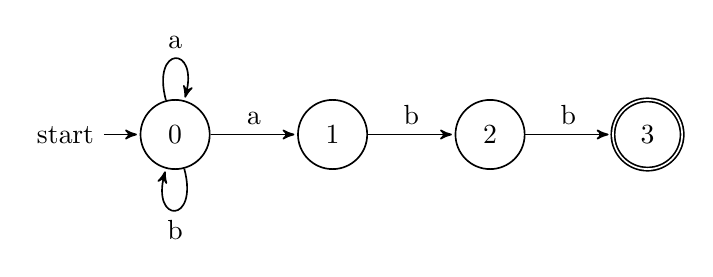
\begin{tikzpicture}[
    % Default arrow tip
    ->,>=stealth',shorten >=1pt,auto,
    % Default node distance
    node distance=2cm,
    % Edge stroke thickness: semithick, thick, thin
    semithick
    ]

    \newState{0}{$0$}{initial}{}
    \newState{1}{$1$}{right of=0}{}
    \newState{2}{$2$}{right of=1}{}
    \newState{3}{$3$}{right of=2}{accepting} 

    \newTransition{0}{0}{a}{loop above}
    \newTransition{0}{0}{b}{loop below}
    \newTransition{0}{1}{a}{}
    \newTransition{1}{2}{b}{}
    \newTransition{2}{3}{b}{}
  \end{tikzpicture}
  \caption{Transition Diagram, accepting the pattern  $(a | b)* abb$ 
  \label{fig:td}}
  \end{figure}

\begin{example}[RegExp to Transition Table] \label{regexp2tt}
\cite{Aho2006}\\
Given the regular expression from \cref{regexp2td} it can be converted into transition table shown in \cref{fig:tt}
\end{example}
\begin{figure}[h!]
  \centering
  \begin{tabular}{| c | c c c |}
    \hline
    \hline
    State & a & b & $\epsilon$\\
    \hline
    0 & $\{0, 1\}$ & $\{0\}$ & $\emptyset$ \\
    1 & $\emptyset$ & $\{2\}$ & $\emptyset$ \\
    2 & $\emptyset$ & $\{3\}$ & $\emptyset$ \\
    3 & $\emptyset$ & $\emptyset$ & $\emptyset$ \\
    \hline
  \end{tabular}
  \caption{Transition Table representation of regular expression in 
        \cref{regexp2td} \label{fig:tt}}
\end{figure}
Transition tables has the advantage that they have an quick lookup time. But 
instead it will take allot of data space, when the alphabet is large. Most 
states do not have any moves on most of the input symbols. \cite{Aho2006}
\subsubsection{Deterministic Finite Automata}
DFA is a special case of an NFA where,
\begin{enumerate}
  \item there are no moves on input $\epsilon$ and
  \item for each state $s$ and input symbol $a$, there is exactly one edge out
        of $s$ labelled with $a$.
\end{enumerate}
While NFA is an abstract representation of an algorithm to recognise the string 
of a language, the DFA is a simple concrete algorithm for recognising strings. 
Every regular expression can be converted in to a NFA and every NFA can be 
converted in to a DFA. \cite{Aho2006} It is the DFA that is implemented and 
used when building lexical analysers. 
\begin{example}[DFA representation of RegExp] \label{regexp2dfa}
\cite{Aho2006}\\
A DFA representation of a regular expression from \cref{regexp2td} is shown in \cref{fig:dfa}
\end{example}
\begin{figure}[!h]
  \centering
  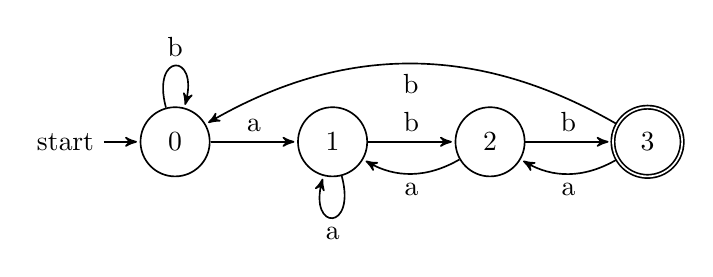
\begin{tikzpicture}[
    % Default arrow tip
    ->,>=stealth',shorten >=1pt,auto,
    % Default node distance
    node distance=2cm,
    % Edge stroke thickness: semithick, thick, thin
    semithick
    ]

    \newState{0}{$0$}{initial}{}
    \newState{1}{$1$}{right of=0}{}
    \newState{2}{$2$}{right of=1}{}
    \newState{3}{$3$}{right of=2}{accepting} 

    \newTransition{0}{0}{b}{loop above}
    \newTransition{0}{1}{a}{}
    \newTransition{1}{1}{a}{loop below}
    \newTransition{1}{2}{b}{}
    \newTransition{2}{3}{b}{}
    \newTransition{2}{1}{a}{bend left}
    \newTransition{3}{2}{a}{bend left}
    \newTransition{3}{0}{b}{bend right}
  \end{tikzpicture}
  \caption{DFA, accepting regular expression in \cref{regexp2td}
  \label{fig:dfa}}
\end{figure}

 

\chapter{Divide-and-Conquer Lexer}
An incremental divide and conquer lexer works by dividing the sequence, to be lexicaly analysed,
into smallest part and analyse them; and then combining them. In the base
case the lexical analysis is done on a single character. The conquer step is
then to combine the smaller tokens into as large tokens as possible. The end
result should be a sequence of token that represent the code. How this is done
will be described below.

\section{Divide and Conquer in General}
This section will try to give a idea of how the Divide and Conquer algorithm works in a general case. So when talking about the incremental lexer there is an understanding about the underlying techniques.

\subsection{The Basics}
The general idea of a divide and conquer is to divide a problem into to smaler parts and solve them separatly and then combine the results. 
A Divide and Conquer algorithm always consist of a pattern with these three steps \cite{Goodrich}.
\begin{description}
\item[Divide:] If the input size is bigger than the basecase then divide the input into subproblems. Otherwise solve the problem using a straightforward method.
\item[Recur:] Recursively solve the subproblems associated with the subset.
\item[Conquer:] Given the solutions to the subproblem, merge them into to the original problem.
\end{description}

\subsection{Associative Function}
The associative property stated for when an expression containing two or more of the same operator, or function, in a row. The order of which of the operations that are executed first has no impact on the result. 

In divide and conquer this is essential. On the conquer step in the divide and conquer algorithm, there is no certain order of which how the subproblems are going to be conquered. So the result of running any part with another part must give the same result as doing it in any other way.

\subsection{Time Complexity}
To calculate the running time of an divide and conquer algorithm the master method can be applied \cite{Cormen}. This method is based on the following theorem.

\begin{theorem}[Master Theorem \cite{Cormen} \label{MasterTheo}] $ $\\
Assume a function $T_n$ constrained by the recurrence
\begin{center}
$T_n = aT_{\frac{n}{b}}+ f(n)$
\end{center}
This is typically the equation of a divide-and-conquer algorithm, where $a$ is the number of sub-problems at each recursive
step, $n/b$ is the size of each sub-problem, and $f(n)$ is the running
time of dividing up the problem space into $a$ parts, and combining
the sub-results together.\\
If we let $e = log_b a$, then
\begin{center}
\begin{tabular}{r c l l}
1. $Tn$ & $=$ & $\Theta(n^{e})$ &  if $f(n) = O(n^{e - \epsilon}$ and $\epsilon > 0$\\
2. $Tn$ & $=$ & $\Theta(n^{e} log n)$ & if $f(n) = \Theta(n^e)$\\
3. $Tn$ & $=$ & $\Theta(f(n))$ & \begin{minipage}[t]{0.6 \columnwidth}
  if $f(n) = \Omega(n^{e+\epsilon})$ and $\epsilon > 0$ and $a \cdot f(n/b) \leq c \cdot f(n)$ where $c < 1$ and all sufficiently large $n$
  \end{minipage}
\end{tabular}
\end{center}
\qeda
\end{theorem}

\subsection{Hand on Example}
The divide and conquer pattern can be preformed on different sorts of algorithm that solves different problems. A general problem is sorting, or more precies sorting a list of integers. This example will show merge-sort.

\begin{enumerate}
\item The algorthim starts with the divide step. Givien the input $S$ the algorithm will check if $S$ consist of a number of elements less or equal to 1.
\begin{itemize}
\item If this is true, return the sequence. A sequence of one or zero elements is always sorted.  
\item If this is false, split the sequence into two (as close as possible) equaly big sequences. $S_1$ and $S_2$, $S_1$ is equal $S$.getRange($1$, $n/2$).
$S_2$ is equal $S$.getRange($(n/2)+1$, $n$). The indexing of the sequence starts at $1$.
\end{itemize}
\item The next step is to sort the subsequences $S_1$ and $S_2$. This is done by recursively call it self with the subsequences as input. There will be 2 calls, one with $S_1$ as input and one with with $S_2$ as input.
\item The to sequences $S_1$ and $S_2$ is has now be recursively sorted and can be merged. Assign $S$ to the result of the merging.
\end{enumerate}
Algortihm~\ref{Alg:MergSort} shows a more formal definition of merge-sort.

\begin{algorithm}
\DontPrintSemicolon
\KwData{Sequence of integers $S$ containing $n$ integers}
\KwResult{Sorted sequence $S$}
\If {$length(S) \leq 1$}{
  \Return $S$ \;
}
\Else {
  $(S_1,S_2) \gets splitAt(S,n/2)$ \;
  $S_1 \gets MergeSort(S_1)$\;
  $S_2 \gets MergeSort(S_2)$\;
  $S \gets Merge(S_1, S_2)$\;
  \Return $S$
}
\caption{MergeSort}
\label{Alg:MergSort}
\end{algorithm}

Given the mergesort algorithm, time complexity is calculated this way.
There are $2$ recurrsive calls, the subproblems are $1/2$ of the original problem size. To merge the two sorted subproblems the worst case is to check every element in the two list, $2 \cdot n/2 = n$. 
\begin{center}
 $T(n) = 2T(n/2) + n$.
\end{center}
Results in: 
\begin{center}
$a = 2$, $b = 2$ and $f(n) = n \;
\Rightarrow n^{log_b a} = n^{log_2 2} = n$
\end{center}
Case 2 of the master theorem applies, since
\begin{center}
$f(n) = O(n)$
\end{center}
So the solution will be:
\begin{center}
$T(n) = \Theta(n^{log_2 2} \cdot log n) = \Theta(n \cdot log n)$
\end{center}

\section{Divide and Conquer Lexing in General}
This section will give a general view of the techniques for an incremental
divide and conquer lexer. Also an overview why it is a good idea using these
techniques, before going into deep details about the incremental lexer this
report relates to.

\subsection{Treestructure}
The incremental divide and conquer lexer should use a structuer where the
code-lexemes can be related to its tokens, current result can be saved and easy
recalculated. A divide and conquer lexer should therefore use a tree structure
to save the lexed result in. Since every problem can be divided in to several
subproblems, until the basecase is reached. This is cleraly a tree structure of
solutions, where the leafs are the tokens for a single character. and the root
is a sequence of all tokens in the code.  

\subsection{Transition map}
To be able to make a divide-and-conquer lexer work you can use a transition map
for the subexpression that has currently been lexed. That is you store for each
subexpression a list of tuples which are built up of an in state, a list of
tokens and an out state. This could in haskell look something like this.
\begin{verbatim}
type Transition = (State,[Tokens],Suffix,State)
type Transitions = [Transition]
\end{verbatim}
\paragraph{The States}
\paragraph{List if Tokens}
\paragraph{The Suffix}

\subsection{The Base Case}
When the lexer tries to lex one character it will create a transition
table using the DFA for the language. It will for each state in the DFA lookup
what out state the character would yield and create a Tokens type of Single.
For the character '/' part of a transition map might look like the following.
\begin{center}
$\left[\begin{array}{ccc}
10&Single '/'&10\\
11&Single '/'&NoState\\
12&Single '/'&10\\
\end{array}\right]$
\end{center}
The reason we keep track of $NoState$ will be evident once we show how the
conquer step work.

\subsection{Conquer Step}
The most general case is a naive lexer that takes the first accepting state it
can find. When two lists of tokens are combined there are two different outcomes:
\begin{description} 
  \item[Concat:]create two tokens if the
    out state of the first list is accepting then the second list will be appended
    to the first list.
  \item[Combine:]The other case is when the first list of tokens does not end
    in an accepting state. In this case the lexer will try to find an in state in
    the second list that is the same as the out state of the first transition.
\end{description}
\begin{center}
$\left[\begin{array}{ccc}
0&Single '/'&1\\
1&Single '/'&Accepting 5\\
\end{array}\right] `combineTokens`
\left[\begin{array}{ccc}
0&Single '/'&1\\
1&Single '/'&Accepting 5\\
\end{array}\right] =
\left[\begin{array}{ccc}
0&Single '//'&Accepting 5\\
1&Multiple '/' [] '/'&Accepting 1\\
\end{array}\right]$
\end{center}
This won't work as a lexer for most languages since it will lex a variable to
variables where the length is a single character, for example ``os'' will be
lexed as two tokens, ``o'' and ``s''. To solve this some more work is needed to
be done.

\subsection{Longest Match}
Instead of taking the naive aproach where a token is created if the lexer finds an
accepting state, the rule for creating a new token will instead be when the
combination of two transitions yields $NoState$ the lists will be appended. That
is, when there is an out state from the first transition that corresponds to an
in state of the second transition and the out state of the second transition
isn't $NoState$, the last token of the first transition and the first token of
the second transition will become one token, otherwise append the second list to
the first list.
%When two list of tokens are combined there are two cases that can emerge. The
%first being that a transition from the first list has an out state that
%corresponds to an in state with a valid out state, i.e. not $NoState$, in the
%second list of transitions. In this case the sufix of the first transition will
%be paired with the prefix of the second and seen as a complete token.
\begin{center}
$\left[\begin{array}{ccc}
0&Single '//'& Accepting 5\\
1&Multiple '/' [] '/' &1\\
\end{array}\right] `combineTokens` 
\left[\begin{array}{ccc}
0&Single '\textbackslash n'&Accepting 6\\
1&Single '\textbackslash n'&1\\
5&Single '\textbackslash n'&NoState\\
\end{array}\right] =
\left[\begin{array}{ccc}
0&Multiple '//' [] '\textbackslash n'&Accepting 6\\
1&Multiple '/' [] '/\textbackslash n'&1\\
\end{array}\right]$
\end{center}
The second case is when the out state for the right token list is $NoState$.
This means that the two lists of tokens can't be combined. In this case the
first token in the second list will be viewed as the start of a token and the
last token in the first list will be viewed as the end of a token.

\begin{figure}[!htp]
\centering
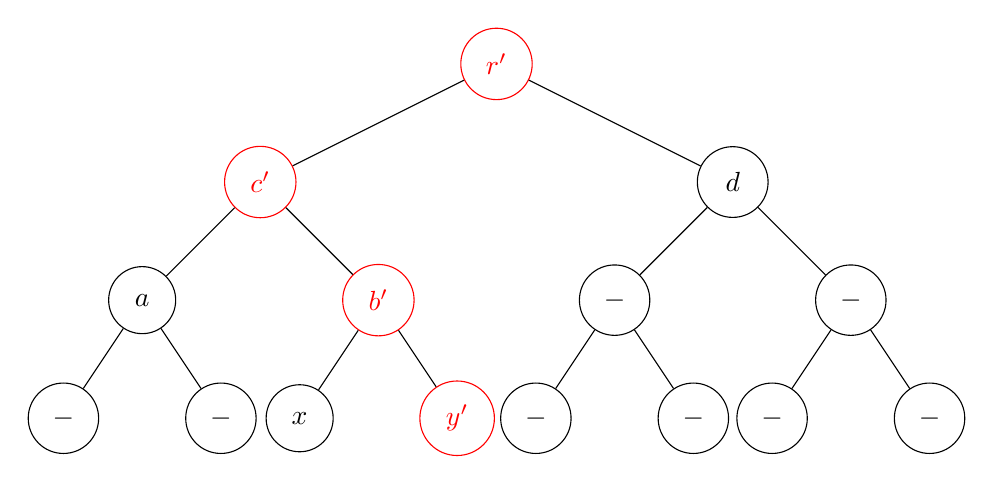
\begin{tikzpicture}[level/.style={sibling distance=60mm/#1, align=center, text centered}]
\node [circle,red,draw, text width = 1.5em, text centered] (z){$r'$}
  child {node [circle,red,draw, text width = 1.5em] (a) {$c'$}
    child {node [circle,draw, text width = 1.5em] (b) {$a$}
      child {node [circle,draw, text width = 1.5em] (c) {$-$}} 
      child {node [circle,draw, text width = 1.5em] (d) {$-$}}
    }
    child {node [circle,red,draw, text width = 1.5em] (e) {$b'$}
      child {node [circle,draw, text width = 1.5em] (f) {$x$}}
      child {node [circle,red,draw, text width = 1.5em] (g) {$y'$}}
    }
  }
  child {node [circle,draw, text width = 1.5em] (i) {$d$}
    child {node [circle,draw, text width = 1.5em] (j) {$-$}
      child {node [circle,draw, text width = 1.5em] (k) {$-$}}
      child {node [circle,draw, text width = 1.5em] (l) {$-$}}
    }
    child {node [circle,draw, text width = 1.5em] (m) {$-$}
      child {node [circle,draw, text width = 1.5em] (n) {$-$}}
      child {node [circle,draw, text width = 1.5em] (o) {$-$}}
    }
  };
\end{tikzpicture}
\caption{Incremental Computing, the updated nodes when a leaf changes \label{fig:incUp}}
\end{figure}

\subsection{Incremental Computing}
To be incremental means that, whenever some part of the data to the algorithm changes the algorithm tries to save time by only recomputing the changed data and the parts that depend on this changed data. \cite{incrementalDef}

For a divide and conquer lexer this would mean only recompute the changed token and the token to the right of the changed token. This is done recurrsivly until the root of the tree is reached. The expected result of this would be that when a character is added to the code of 1024 tokens, instead of relex all 1024 tokens the lexer will only do 10 recalculations for new tokens. Since, $log_2 1024 = 10$. This can be explained by the \cref{MasterTheo}. How this is calculated for an incremental divide and conquer lexer is described more in detail in the next sub-section.

\subsection{Expected Time Complexity}
Since incremental computing stated that only content which depends on the new data will be recalculated. That is, follow the branch of the tree from the new leaf to the root and recalculated every node on this path. 
As shown by \cref{fig:incUp}. Only one subproblem is updated in every level of the tree. Back to the master theorem. Let put this in to numbers, $e = log_b a$ where $a$ is number of recursive calls and $n/b$ is size of the subproblem where $n$ is the size of the original problem. As shown by the \cref{fig:incUp} number of needed update calls is $1$, therefor $a = 1$. The constant $b$ is still $2$. This will give $e = log_2 1 = 0$. Thus the update function of the incremental algorithm will have a time complexity of $\Theta(n^0 \cdot log n) = \Theta(log n)$

\section{Pitfalls}
This section will describe techniques that were tried under the constuction of 
the incremental divide and conquer lexer but was shown to give bad results.

\subsection{Brutefore}
The first naive solution was to "bruteforce" to find the lex. This was showned to be to resource-eating. But it describes the general idea of how the problem could be solved. Why it was a bad solution will be described futher on in the text. 

The above rules will work for very simple languages. When comments are
introduced you will get the problem that the whole code can be one long partial
comment token. To remedy this you can add two rules:
\begin{itemize}
\item Every time you combine two tokens you only do so if the combination has a
transition from the starting state.
\item If two tokens can be combined completly, check if the next token can be
combined aswell.
\end{itemize}
This ensures that every token starts in the starting state and that each token
is as long as it can be.

This also has some problems though. When keywords like ``else if'' are
introduced the lexer will start to lex like in \cref{elseif}. To solve this the
lexer checks when two tokens are completely uncombinable if the first of these
have an accepting state as outgoing state. If the token don't have an accepting
out state, the lexer tries to break up the token until it does. The exception to
this rule is single characters which are permitted to not have no accepting out
states.
\begin{example}[else if lexing]\label{elseif}
Somewhere in the middle of the code ``... 1 else 0 ...''
\begin{center}
\begin{tabular}{ll}
String & Type\\
1 & $Number$\\
\_ & $Space$\\
else\_ & $Nothing$\\
0 & $Number$\\
\end{tabular}
\end{center}
\end{example}

\begin{example}[Devide and Append]
The lexer will always try to build as lage tokens as possible. When it realizes that this cant be done it has to backup and try to combine the parts in a different way. This example will show how this is done in theory. 

The code segment for this example is: 
\begin{center}
"else return".
\end{center}
The tree in \cref{fig1:elseif} shows the first step of the token combine rutine. Clearly this returns a nonexsisting token. 
\begin{figure}[h!]
  \centering
  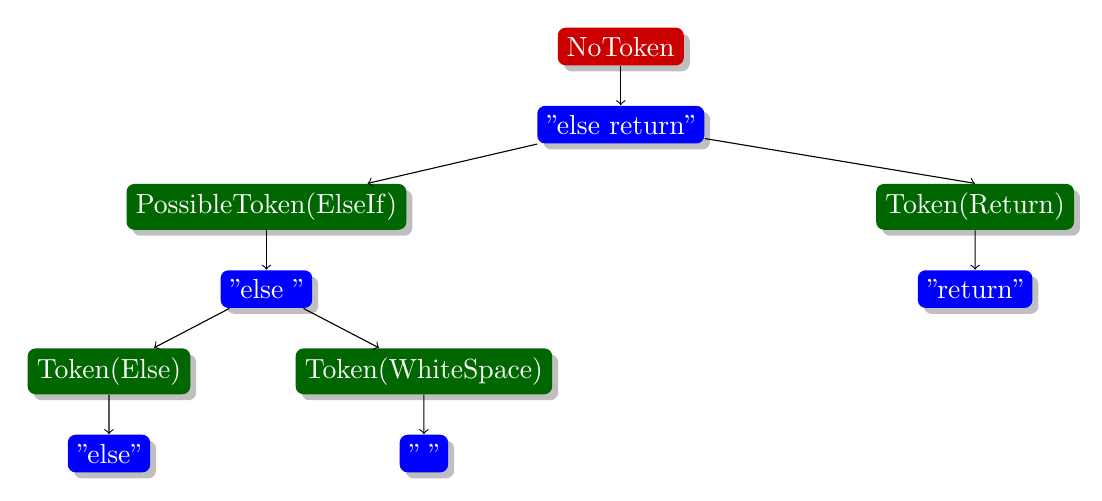
\begin{tikzpicture}[
    error/.style={rectangle, draw=none, rounded corners=1mm, fill=black!20!red, drop shadow,
        text centered, anchor=north, text=white},
    fact/.style={rectangle, draw=none, rounded corners=1mm, fill=black!60!green, drop shadow,
        text centered, anchor=north, text=white},
    state/.style={rectangle, draw=none, rounded corners=1mm, fill=blue, drop shadow,
        text centered, anchor=north, text=white},
    leaf/.style={rectangle, draw=none, rounded corners=1mm, fill=blue, drop shadow,
        text centered, anchor=north, text=white},
    level distance=0.5cm, growth parent anchor=south
    ]
    \node (State00) [error] {NoToken} [->]
        child{ [sibling distance=9cm]
            node (State01) [state] {"else return"}
            child{
                node (Fact02) [fact] {PossibleToken(ElseIf)}
                child{ [sibling distance=4cm]
                    node (State02) [state] {"else "}
                    child{
                        node (Fact03) [fact] {Token(Else)}
                        child{
                            node (State03) [leaf] {"else"}
                        }
                    }
                    child{
                        node (Fact04) [fact] {Token(WhiteSpace)}
                        child{ [sibling distance=1.2cm]
                            node (State04) [leaf] {" "}
                        }
                    }
                }
            }
            child{ [sibling distance=4cm]
                node (Fact05) [fact] {Token(Return)}
                child{
                    node (State05) [leaf] {"return"}
                }
            }
        }
    ;
  \end{tikzpicture}
  \caption{Lexer thinks "else " is an "else if" pattern. 
  \label{fig1:elseif}}
\end{figure}
From here when the lexer has found that there are no tokens for this lexeme it will try to split the left child token.
\begin{center}
    split("else ") => ["else"," "]
\end{center} 
Now the lexer has a pair of two lexems that represent valid tokens. The lexer knows that combinding these two lexems in the pair returns in a NoToken result. So The only thing to do is to try to combine the right token in the pair with the right child token and let the token to the left in the pair stand alone. 
\begin{figure}[!h]
  \centering
  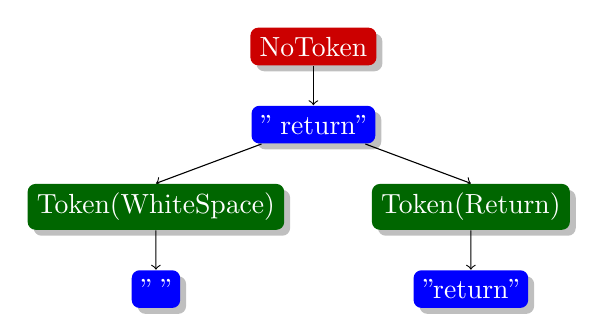
\begin{tikzpicture}[
    error/.style={rectangle, draw=none, rounded corners=1mm, fill=black!20!red, drop shadow,
        text centered, anchor=north, text=white},
    fact/.style={rectangle, draw=none, rounded corners=1mm, fill=black!60!green, drop shadow,
        text centered, anchor=north, text=white},
    state/.style={rectangle, draw=none, rounded corners=1mm, fill=blue, drop shadow,
        text centered, anchor=north, text=white},
    leaf/.style={rectangle, draw=none, rounded corners=1mm, fill=blue, drop shadow,
        text centered, anchor=north, text=white},
    level distance=0.5cm, growth parent anchor=south
    ]
    \node (State00) [error] {NoToken} [->]
        child{ [sibling distance=4cm]
            node (State01) [state] {" return"}
            child{ [sibling distance=4cm]
                node (State02) [fact] {Token(WhiteSpace)}
                child{
                    node (Fact02) [leaf] {" "}
                }
            }
            child{ [sibling distance=4cm]
                node (Fact03) [fact] {Token(Return)}
                child{
                    node (State03) [leaf] {"return"}
                }
            }
        }
    ;
  \end{tikzpicture}
  \caption{Lexer tries to combine an white space with a return statement
  \label{fig4:elseif}}
\end{figure}
This also return a NoToken. So the same thing will be done again. The lexer tries to split the left child before NoToken was given. In this case the whitespace. 
\begin{center}
split(" ") => []
\end{center}
But becouse the whitespace is of the lowest form and is not build up by smaller tokens the resulting list from the split function will be empty. Now the lexer knows that this token must be by it self. The "return" is the last lexeme in this example code so the lexer can't combine it futher. Thus the lexer has found the resulting sequence of tokens:
\begin{center}
    [(Token(Else), "else"), (Token(WhiteSpace)," "), (Token(Return), "return")]
\end{center} 
\end{example}

\subsection{Dont know what to call this!}
When the code is divided the lexer doesn't know if the string (or character) it
lexes is the first, last or is somewhere in the middle of a token. Instead of
checking what type of token the string will be (if it were to begin from the
starting state) it saves all the possible state transitions for that string.

In the examples that follow below state 0 is considered the starting state and
state $1-6$ are considered accepting.
\begin{example}[Transition map for a token]\label{transMap}
A hypothetical transition map for the char 'i'.
\begin{center}$\begin{array}{cc}
\multicolumn{2}{c}{'i'}\\
in & out\\
0 & 1\\
1 & 1\\
8 & 7\\
\end{array}$\\
\end{center}
\end{example}
In the base case the lexer will map all the transitions for all individual
characters in the code and construct partial tokens of them. The conquer step
will then combine two of these at a time by checking which possible outgoing
states from the first token can be matched with incoming states from the second
token. If there are such pairs of outgoing states with incomming states, then a
new partial token is created.
\begin{example}[Combining two tokens]\label{combTok}
'if' can be an ident (state 1) or part of 'else if' (state 5).
\begin{center}$\begin{array}{cc}
\multicolumn{2}{c}{'i'}\\
in & out\\
\textcolor{brown}{0} & \textcolor{brown}{1}\\
1 & 1\\
\textcolor{blue}{8} & \textcolor{blue}{7}\\
\end{array}
`combineToken`
\begin{array}{cc}\multicolumn{2}{c}{'f'}\\
in & out\\
0 & 1\\
\textcolor{brown}{1} & \textcolor{brown}{1}\\
\textcolor{blue}{7} & \textcolor{blue}{5}\\
\end{array}
=
\begin{array}{cc}\multicolumn{2}{c}{'if'}\\
in & out\\
\textcolor{brown}{0} & \textcolor{brown}{1}\\
\textcolor{blue}{8} & \textcolor{blue}{5}\\
\end{array}$\\
\end{center}
\end{example}
If there are no pairs of outgoing states which match the incomming states the
lexer will try to combine the first token with as much of the second token as
possible. In this case there will be a remainder of the second token, The lexer
can now be sure that the begining of the remainder is the begining of a token
and that the merged part is the end of the token before.
Since the lexer knows the remainder is the begining of a token it strips all
transitions but the one that has incomming state as starting state. Since the
start token is the end of a Token it strips all but the transitions ending in an
accepting state.
\begin{example}[Combining a token a part of the second token]\label{combSplit}
'ie' ends in the accepting state for ident (1) and '\_' starts in the
starting state.
\begin{center}
$\begin{array}{cc}\multicolumn{2}{c}{'e\_'}\\
in & out\\
\textcolor{brown}{10} & \textcolor{brown}{8}\\
\end{array}
=
\begin{array}{cc}\multicolumn{2}{c}{'e'}\\
in & out\\
0 & 11\\
\textcolor{blue}{1} & \textcolor{blue}{1}\\
6 & 1\\
\textcolor{brown}{10} & \textcolor{brown}{9}\\
\end{array}
`combineToken`
\begin{array}{cc}\multicolumn{2}{c}{'\_'}\\
in & out\\
0 & 2\\
2 & 2\\
\textcolor{brown}{9} & \textcolor{brown}{8}\\
\end{array}
$\\
$\begin{array}{cc}
\multicolumn{2}{c}{'i'}\\
in & out\\
\textcolor{blue}{0} & \textcolor{blue}{1}\\
\textcolor{blue}{1} & \textcolor{blue}{1}\\
8 & 7\\
\end{array}
`combineToken`
\begin{array}{cc}\multicolumn{2}{c}{'e\_'}\\
in & out\\
10 & 8\\
\end{array}
=
\begin{array}{cc}\multicolumn{2}{c}{'ie'}\\
in & out\\
\textcolor{blue}{0} & \textcolor{blue}{1}\\
\textcolor{blue}{1} & \textcolor{blue}{1}\\
\end{array} ++ 
\begin{array}{cc}\multicolumn{2}{c}{'\_'}\\
in & out\\
0 & 2\\
\end{array}$\\
\end{center}
\end{example}
\# Perhaps remove this part\\
However the remainder may not have the start state as a possible incomming state.
In this case the lexer tries to find the largest possible token (that has the
starting state as incomming state) and tries to construct a token of the rest of
the remainder, repeating this procedure until the entire remainder has been
split into acceptable tokens. All the tokens accept the one that is on the very
end of the sequence will have all but their accepting states stripped. This case
does occur quite frequently since most languages has comments and strings which
can contain anything.
\begin{example}[Handling the remainder]\label{remToken}
'\_' starts in the starting states and ends in an accepting state and 'e' starts
in the starting state, it doesn't have to end in an accepting state.
\begin{center}
$\begin{array}{cc}\multicolumn{2}{c}{'\_i'}\\
in & out\\
\textcolor{brown}{9} & \textcolor{brown}{7}\\
\end{array}
=
\begin{array}{cc}\multicolumn{2}{c}{'\_'}\\
in & out\\
0 & 2\\
2 & 2\\
\textcolor{brown}{9} & \textcolor{brown}{8}\\
\end{array}
`combineToken`
\begin{array}{cc}
\multicolumn{2}{c}{'i'}\\
in & out\\
0 & 1\\
1 & 1\\
\textcolor{brown}{8} & \textcolor{brown}{7}\\
\end{array}$\\
$checkRemainder \left(\begin{array}{cc}\multicolumn{2}{c}{'\_i'}\\
in & out\\
9 & 7\\
\end{array} \right)
=
\begin{array}{cc}\multicolumn{2}{c}{'\_'}\\
in & out\\
0 & 2\\
\end{array} ++
\begin{array}{cc}\multicolumn{2}{c}{'i'}\\
in & out\\
0 & 1\\
\end{array}$\\
\end{center}
\end{example}
When all partial tokens has been combined in this way the resulting sequence of
tokens represents the the code the lexer was run on.

\section{Lexical Errors}
Since the lexer has to be able to handle any kind of possible not "complete"
tokens, error handling can be done in different ways. One approach is to simply
return as many tokens as possible from the code and where there might be lexical
errors the lexer returns the error in as small parts as possible.

\begin{example}[A lexer that only lexes letters] When the lexer encounters the
string "what @ day" it would return:
\begin{center}
\begin{tabular}{ll}
String & Type\\
What & $Word$\\
'\_' & $Space$\\
'@' & $No\_Token$\\
'\_' & $Space$\\
day & $Word$\\
\end{tabular}
\end{center}
\end{example}

\chapter{Parallelism}
\# Our solution should be able to run on several cores. 
This chapter shoul be about why how and so on.

\chapter{Implementation}\label{chap:imp}
In this chapter the tools, data structure and implementation of the incremental
divide and conquer lexer is explained. The implementation of the incremental
divide and conquer lexer uses fingertrees for storing the intermediate tokens
and the lexed text. It has an internal representation of the tokens to keep
track of the data needed when two fingertrees are combined. The lexical routines
for combining the internal token data type take advantage of functional
composition in order to get lazy updating of the tokens when two fingertrees are
combined. The complete implementation can be found in \cref{chap:code}.

%\section{Alex}
\section{The DFA Design}
The DFA used in the incremental lexer was created using Alex. Alex is a Haskell
tool for generating lexical analyzers given a
description of the language in the form of regular expressions, it is similar to
lex and flex in C and C++. The resulting lexer is Haskell 98 compatible and can
easily be used with the parser Happy, a parser generator for Haskell \cite{alex}.
Alex is notably used in BNFC which is a program to generate among other things a
lexer, parser and abstract syntax from Backus-Naur Form \cite{bnfc}.

The reason for using Alex to generate the DFA is that it optimizes the number of
elements in the transition table. Instead of
having an array for every possible character and state combination, 5 arrays are
generated that takes advantage of the fact that for most characters the same
state will be used the majority of time. This saves a lot of elements that
would otherwise be the same in the array.

\newpage

The trade off for using the Alex generated DFA is that some minor arithmetic
operations are used and some extra lookups are needed. These operations
are far less time consuming then the rest of the lexical operations.

\section{Token data structure}
To keep all the information that might be needed when combining two texts, a data
structure for the tokens was created. This data type contains more information
about the last token than what a sequential lexer would save, exactly what is
explained in \cref{sub:suff}.

%Rewrite this paragraph.
Since this project is about creating a real-time lexing tool, performance is
important. Therefore there are advantages of using sequences instead of lists,
since they have better time complexity. The most notable place where this is
used is in the measure of the fingertree, where the tokens are stored in a
sequence rather then a list. Sequences are also used elsewhere in the project
but the measure is the most notable place since it is frequently updated.

\subsection{Tokens}
The internal structure used to store lexed tokens is called $Tokens$. There are
three constructors in the $Tokens$ data type, see \cref{fig:tokens}.

\begin{figure}[h!]
  \lstinputlisting[language=Haskell]{examples/Token.hs}
  \caption{Tokens Data Type\label{fig:tokens}}
\end{figure}

$NoTokens$ is a representation of when an empty string has been lexed.
$InvalidTokens$ represents a lexical error somewhere in the text that was lexed,
the sequence of characters is the lexical error or last token lexed. The
$Tokens$ constructor is the case when legal tokens have been found. $currentSeq$
are all the currently lexed tokens save for the last, $lastToken$ are all the
possible ways that the last token can be lexed, in this implementation this is
referred to as the suffix and what it is and why it is needed will be explained
next.

\subsection{Suffix}\label{sub:suff}
When a text is lexed it is uncertain that the last token is the actual end of
the file since it may be combined with something else. To ensure that all
possible outcomes will be handled the last token can take one of three
different forms. The part of the text lexed can end in:
\begin{itemize}
\item a state that is not accepting,
\item an accepting state,
\item a state that is not accepting, but the text can also be a sequence
  of multiple tokens.
\end{itemize}
To keep track of these cases a data structure that captures them was
implemented, see \cref{fig:suff}.

\begin{figure}[h!]
  \lstinputlisting[language=Haskell]{examples/Suffix.hs}
  \caption{Suffix Data Type\label{fig:suff}}
\end{figure}

The $Str$ constructor is used to keep track of partially complete tokens, an
example of this is when a string is started but the end quotation character have
not yet been found.

The $One$ constructor is used when exactly one token has been found, it may or
may not be the token that is used in the final result of the lexing. Since this
constructor is a special case of the $Multi$ constructor it can be omitted.
However the $One$ constructor makes certain cases redundant since the lexer
makes assumptions that can not be made for the $Multi$ constructor.

The $Multi$ constructor is used when at least one token has been found but the
lexeme for the suffix does not match exactly one token. The entire suffix still
needs to have an out state. This type of suffix can typically be found when
the beginning of a comment is lexed. for example the text \emph{/*hello world}
would be lexed to a sequence of complete tokens, ``/'', ``*'', ``hello'' and
``world'', but the lexer still needs to keep track of the fact that it may be in
the middle of a multi-line comment. Note that in this case the $Tokens$ data
structure would have one out state, the state for the middle of a comment, and
the suffix would have another, the end of an ident.

\section{Transition Map}
The transition map is a function from an in state to $Tokens$. As shown in
\cref{fig:tokens} the $Tokens$ data type contains the out state.

\begin{figure}[h!]
  \lstinputlisting[language=Haskell]{examples/Transition.hs}
  \caption{Transition Data Type \label{fig:transition}}
\end{figure}

This data type is used in the lexical routines. The reason for using transition
maps is that the lexer does not know what the in state for a lexed text is, hence
the tokens for all possible in states must be stored. The transition map can be
implemented in two ways, a table format and a function composition format.

The table format uses an array to store the currently lexed tokens where the
index of the array represents the in state for that sequence of tokens. This is
useful when the tokens need to be stored since it ensures that the tokens are
computed.

When combining lexed tokens it is useful to use functional composition since it
ensures that no unnecessary states will be computed. The drawback is that it
does not guarantee that the actual tokens are computed which may result in slow
performance at a later stage in the lexing. Since Haskell does not evaluate
functional composition to $(f . g) x$ but rather $f (g~x)$ all incrementality
will be lost with this data structure.

Both these representations are used in the incremental divide and conquer lexer.
The table format is used when storing the tokens in the fingertree to allow for
fast access and incrementality. The function composition is used when combining
tokens to ensure that only needed data is computed.

\section{Fingertree}
The fingertree is constructed with the characters of a text being the leaves and
with the table format transition map as it is measure. The $Table$ data type has
to be a monoid in order to be a legal measure of the fingertree.

\begin{figure}[h!]
  \lstinputlisting[language=Haskell]{examples/Fingertree.hs}
  \caption{The data type for storing the tokens and text \label{fig:fingertreedt}}
\end{figure}

The monoid class in Haskell has two different functions, $mempty$ which is the
identity element and $mappend$ which is an associative operator that describes
how two elements are combined. As can be seen in \cref{fig:tablemonoid},
$mempty$ creates an array filled of empty $Tokens$. $mappend$ extracts the
functions from the old tables, combines them using $combineTokens$ then creates
a new table filled with the combination.

\begin{figure}[h!]
  \lstinputlisting[language=Haskell]{examples/TableMonoid.hs}
  \caption{The tabulate functions and monoid implementation \label{fig:tablemonoid}}
\end{figure}

There are two helper functions that convert between the table format that is
stored as the measure and the function composition format that is used in the
lexical routines. These can be seen in \cref{fig:tablemonoid}.

\section{Lexical routines}
%\subsection{combineTokens}
The lexical routines are divided into five functions. They each handle
different parts of the lexical steps that are needed in an incremental divide and
conquer lexer.

%\begin{figure}[h!]
%  \lstinputlisting[language=Haskell]{examples/LexicalFunHeads.hs}
%  \caption{Function definitions of the lexical routines \label{fig:funheads}}
%\end{figure}

\subsection{Combination of Tokens}
\begin{figure}[h!]
  \lstinputlisting[language=Haskell]{examples/CombineTokens.hs}
  \caption{The $combineTokens$ function \label{fig:combinetoks}}
\end{figure}

$combineTokens$ is the function called when two fingertrees are combined.
The function starts by checking if the tokens generated from $in\_state$ from
the first transition is empty or invalid in which case the output is trivial. If
the tokens generated are valid, the tokens are passed on to $combineWithRHS$
together with the second transition.

\subsection{Combine Tokens With Right Hand Side}
$combineWithRHS$ checks how the tokens from the first
transition are to be combined with the second transition.

\begin{figure}[h!]
  \lstinputlisting[language=Haskell]{examples/CombineWithRHS.hs}
  \caption{$CombineWithRHS$ function\label{fig:cwrhs}}
\end{figure}

$combineWithRHS$ starts by creating tokens from the second transition, $toks2$,
using the out state from the first tokens, this can result in three different
cases, the definition of the variable names can be found in \cref{fig:cwrhs}.
\begin{description}
\item[isEmpty]If $toks2$ is empty $toks1$ is returned.
\item[isValid]If $toks2$ is valid it means that the last token from the
  $toks1$ can be combined into one token with the first token in $toks2$.
\item[otherwise]If $toks2$ is not valid the lexer checks the suffix of $toks1$
  to see if it ends in an accepting state or a valid state.
  \begin{itemize}
  \item if the $One$ constructor is found the suffix ends in an accepting state
    which means that tokens created from the start state can be appended to
    $toks1$.
  \item If the $Multi$ constructor is found the tokens from the suffix,
    $suffToks$, is extracted and a recursive call to $combineWithRHS$ is made
    with $suffToks$ as argument instead.
  \item If the $Str$ constructor is found the suffix does not end in a valid
    state and $InvalidTokens$ will be returned.
  \end{itemize}
\end{description}
%The switch case for $Multi$ extracts the tokens from the suffix and recursively
%calls \emph{combineWithRHS} to see if there is some other possible way to
%combine the transitions.

\subsection{Merge Two Tokens}
$mergeTokens$ combines the last token from the first tokens with
the first token of the second tokens, for the code see \cref{fig:mergetokens}.

\begin{figure}[h!]
  \lstinputlisting[language=Haskell]{examples/MergeTokens.hs}
  \caption{$MergeTokens$ function \label{fig:mergetokens}}
\end{figure}
\begin{itemize}
\item If there are more then one token in $toks2$, $suff1$ is combined into one
  token with the first token in $toks2$ and the rest of the tokens in $toks2$
  is appended and returned.
\item If there is exactly one token in $toks2$, the suffix from $toks2$ is
  combined with $suff1$. When two suffixes are combined some extra checks are
  needed. If $toks2$ has an accepting out state, the two suffixes
  can be combined into one token. If $toks2$ does not have an accepting out
  state the work is passed on to $mergeSuff$.
\end{itemize}

\subsection{Merging Suffixes}
$mergeSuff$ checks which pairs of suffixes it has and takes the appropriate
actions.

\begin{figure}[h!]
  \lstinputlisting[language=Haskell]{examples/MergeSuff.hs}
  \caption{$MergeSuff$ function \label{fig:msuff}}
\end{figure}
\begin{itemize}
\item If the first suffix is of type $Multi$ the function calls
  $combineWithRHS$. If the resulting tokens is invalid a recursive call is made
  with the suffix from the new tokens as first suffix.
\item If the first suffix is of type $Str$ the result will always be another
  $Str$ no matter what is in the second suffix so the string is extracted and
  appended.
\item if the first suffix is of type $One$ and the second $Str$ a new $Multi$
  suffix is created. A new second tokens is created using the start state on the
  second suffix, if this results in a valid $Tokens$, the token from the first
  suffix is prepended. If it is not valid the $Str$ is just added to the end of
  the new suffix.
\item When both suffix are $One$ they can be combined into a single token.
\item When the first suffix is $One$ and the second is $Multi$ it is passed onto
  $mergeTokens$.
\end{itemize}
\subsection{Append to Sequence of Tokens}
$appendTokens$ checks if there is a lexical error in $toks2$. if there is
an error, that error is returned, otherwise $toks2$ is appended to $toks1$.
\lstinputlisting[language=Haskell]{examples/AppendTokens.hs}

\chapter{Testing}
The incremental lexer has ass mention before three requirements, Robust, Efficient and Precise. To be robustness the lexer don't crash when encounter an error in the syntax. That is, the lexer will find the correct token if the syntactical error is fixed by the user. For it to be efficient the feedback to the user must be instant.
Finally to be precise the lexer must give a correct result. This chapter will talk about how this requirements are tested and if they are fulfilled. 

\section{Robustness}

\section{Efficiency}

\section{Preciseness}
For an incremental lexer to work, the lexer must be able to do lexical analysis of any substring of a code. And come to correct result for that substring. It must also be able to merge any two substrings neighboring in a code and the result of this merge must be the same as lexing the two substrings as one substring.
To test if the lexer is as close as possible to the result done by the compiler the resulting token sequence should be the same sequence given from Alex, a open-source lexer written in Haskell, when lexing the same code-string.
To control this the separate tokens in the resulting sequences are compared for equality. 
This code in \cref{fig:CheckEquility} shows the test for equality:

\begin{figure}[h!]
  \centering
  \lstinputlisting[language=c]{examples/CorrectEquility.hs}
  notEqual function is a function which patter-match on the to different tokens and returns true if they are not of the same type.
  \caption{Code for testing tokens from IncLex is equal to tokens from Alex. 
  \label{fig:CheckEquility}}
\end{figure} 

\subsection{Check Splits}

\subsection{Check Merges} 


%\begin{filecontents*}{time.csv}
%characters*1000, time in microsecs
%n      alex   upd
%1000   210    150
%10000  1901   251
%20000  3910   329
%30000  5303   361
%40000  7079   361
%50000  8933   367
%60000  12140  460
%70000  14860  469
%80000  16850  523
%90000  17170  424
%100000 20920  554
%110000 24960  486
%120000 26430  503
%130000 28420  649
%140000 37890  575
%150000 33790  570
%160000 36850  624
%170000 39860  468
%180000 42570  496
%190000 42410  513
%\end{filecontents*}

\begin{filecontents*}{spacef.csv}
n                        fn
1                        1
10                       29
100                      580
1000                     8987
10000                    123631
100000                   1568946
1000000                  18951445
10000000                 223222809
100000000                2565782300
1000000000               28926258207
10000000000              322820130851
100000000000             3562561046566
1000000000000            38900488372265
10000000000000           422407813955629
100000000000000          4559262511644720
1000000000000000         48874100093157427
10000000000000000        521985601490518071
100000000000000000       5555884811924144186
1000000000000000000      58847078495393153085
10000000000000000000     621553255926290448449
\end{filecontents*}

\begin{filecontents*}{time.csv}
%characters*1000, time in microsecs
n       alex   upd  inc
1000    137    101  8492
10000   1372   174  202100
20000   2794   227  434100
30000   4103   236  498900
40000   5511   243  780100
50000   6935   228  935500
60000   8368   286  1000000
70000   9870   320  1452000
80000   11560  297  1479000
90000   13120  255  2105000
100000  14910  345  2086000
110000  16600  332  2037000
120000  18510  344  2478000
130000  20410  369  2578000
140000  22230  350  2617000
150000  24210  366  2668000
\end{filecontents*}

\begin{filecontents*}{space.csv}
n       size
100     11
200     21
400     40
800     77
1600    259
3200    387
6400    643
12800   1283
25600   2436
51200   4870
102400  9737
204800  19346
409600  38688
819200  77244
1638400 154486
\end{filecontents*}

\chapter{Result}
The incremental lexer has three requirements, it should be
robust, efficient and precise. Robustness means that the lexer does not crash
when it encounter an error in the syntax. That is, if a string would yield an
error when lexed from the starting state the lexer does not return that error but
instead stores the error and lexes the rest of the possible input states since
the current string might not be at the start of the text. The implementation
this report propose is robust since it stores errors in the data structure
rather then returning an error.

For it to be efficient the feedback to the user must be instant, or more
formally the combination of two strings should be handled in $\Theta(log(n))$ time.

Finally to be precise the lexer must give a correct result. This chapter is
describing how these requirements are tested and what the results are.

In the sections below, any mention of a sequential lexer refers to a lexer
generated by Alex using the same Alex file as was used when creating the
incremental lexer \cite{alex}. The reason why Alex was used was because the DFA
generated by Alex was used in the incremental lexer, thus ensuring that only the
lexical routines differs.

\section{Preciseness}
For an incremental lexer to work, the lexer must be able to do lexical analysis
of any part of a text and be able to combine two partial texts. If the lexical
analysis of one partial text does not result in any legal tokens it must be able
to be combined with other partial texts that makes it legal tokens. The lexical
analysis of a text might not always result in the same tokens that the
combination of the text with another text would give.

To test these cases a test was constructed which did a lexical analysis on two
partial texts using the incremental lexer and then combining the results into
one text. The result of the combination should be the same as the lexical
analysis of the entire text using the incremental lexer and the result using a
sequential lexer.

It is not enough to test if the combination of two partial texts yields the
same sequence of tokens as the text. To test that the result of the incremental
lexer was the correct sequence of tokens, it was compared to what a sequential 
lexer generated. This comparison was an equality test that compared token for
token that they were the same kind of token and had the same lexeme.

\cref{fig:CheckEquility} shows the test for equality:
\begin{figure}[h!]
  \centering
  \lstinputlisting[language=c]{examples/CorrectEquility.hs}
  notEqual function is a function which pattern-match on the two different
  tokens and returns true if they are not of the same type.
  \caption{Code for testing tokens from IncLex is equal to tokens from Alex. 
  \label{fig:CheckEquility}}
\end{figure}

Tests were performed on different files that were cut in different places when
the update was tested. In all the tests the incremental lexer produced the same
tokens as the sequential lexer. When these tests were done no text that would
produce a lexical error was used. Some partial texts did produce lexical errors
but the texts passed through the sequential lexer and compared to the result of
the incremental lexer did not produce lexical errors.

%\section{Efficiency}
\section{Performance}
All tests, where time performance was measured, were done with the help of
Criterion, a Haskell library. Criterion has tools to ensure that the functions
being tested is evaluated to normal form. Criterion runs the tests 100 times
with a warm up run by default. The warm up run makes sure that all inputs to the
functions being tested are evaluated before the actual testing begins, this
ensures that nothing but the function being tested is measured \cite{criterion}.

To make sure that the time performance tests were not skewed under a certain
system they were tested on different hardware and operating systems. The results
were similiar on all the systems tested. The results presented below were done
on an intel i5 quad core at 2900MHz with 8GB memory under the linux Red Hat
operating system.

To measure the performance of the incremental step two fingertrees were created,
each representing one half of a text. By creating the two fingertrees the
transition map for the code in those trees are created as well. The benchmarking
was then done on the combination of the two trees. The results of the incremental
lexer benchmarking sugged a running time of $\Theta(log(n))$. To get a reference
point the same text was lexed using a sequential lexer. The benchmarks can be
found in \cref{fig:IncSeqTime} and \cref{fig:IncTime}. More details on the
performance benchmarks can be found in \cref{preformanceAppendix}.

%Tester för nybyggning av träd?
\begin{figure}[!h]
%\begin{center}
\begin{tikzpicture}
    \begin{axis}[
    width=0.7\textwidth,
    height=0.4\textwidth,
    ymajorgrids,
    xmajorgrids,
    title = {Incremental lexer},
    scaled y ticks=real:1,
    scaled x ticks=real:1e3,
    ymin=0,
    xmin=0,
%    x tick label style={/pgf/number format/1000 sep=},
    ytick scale label code/.code={},
    xtick scale label code/.code={},
    ylabel={$\mu s$},
    xlabel={$*1000$ characters},
    legend pos=outer north east
    ]
        \addplot table[x=n,y=upd] {time.csv};\addlegendentry{Incremental update}
    \end{axis}
\end{tikzpicture}
%\end{center}
\caption{Benchmarking times of an incremental update\label{fig:IncTime}}
\end{figure}

\begin{figure}[!h]
%\begin{center}
\begin{tikzpicture}
    \begin{axis}[
    width=0.7\textwidth,
    height=0.4\textwidth,
    ymajorgrids,
    xmajorgrids,
    title = {Update compared to sequential},
    scaled y ticks=real:1e3,
    scaled x ticks=real:1e3,
    ymin=0,
    xmin=0,
%    x tick label style={/pgf/number format/1000 sep=},
    ytick scale label code/.code={},
    xtick scale label code/.code={},
    ylabel={$ms$},
    xlabel={$*1000$ characters},
    legend pos=outer north east
    ]
        \addplot table[x=n,y=upd] {time.csv};\addlegendentry{Incremental update}
        \addplot table[x=n,y=alex] {time.csv};\addlegendentry{Sequential lexing}
    \end{axis}
\end{tikzpicture}
%\end{center}
\caption{Comparison between an incremental update and sequential lexer\label{fig:IncSeqTime}}
\end{figure}

The running time when constructing the tree was not as fast as either the update
or the sequential lexer. The tests for the running time, when constructing a new
tree, sugged $\Theta n\log(n)$, this was expected since there are $\log(n)$
updates for every character. The result can be found in \cref{fig:IncNewTime}.

\begin{figure}[!h]
%\begin{center}
\begin{tikzpicture}
    \begin{axis}[
    width=0.7\textwidth,
    height=0.4\textwidth,
    ymajorgrids,
    xmajorgrids,
    title = {Comparison},
    scaled y ticks=real:1e3,
    scaled x ticks=real:1e3,
    ymin=0,
    xmin=0,
%    x tick label style={/pgf/number format/1000 sep=},
    ytick scale label code/.code={},
    xtick scale label code/.code={},
    ylabel={$ms$},
    xlabel={$*1000$ characters},
    legend pos=outer north east
    ]
        \addplot table[x=n,y=inc] {time.csv};\addlegendentry{Incremental lexing}
        \addplot table[x=n,y=alex] {time.csv};\addlegendentry{Sequential lexing}
    \end{axis}
\end{tikzpicture}
%\end{center}
\caption{Comparison between the sequential lexer and the incremental lexer when
         lexing an entire file\label{fig:IncNewTime}}
\end{figure}

%Since the incremental lexer uses a tree structure there will be an increase in
%data-space used compared to a sequential lexer. Since the root of every partial
%tree stores the lexed tokens for that tree, every level of the tree will store
%approximately the size of the complete tokens for the entire text. A lexer that
%uses a DFA with $m$ states will produce token data structure that grows with
%$\Theta(mn)$ since each in state will have the tokens for that state. The depth
%of the tree is $\log(n)$, this suggest a space complexity of
%$\Theta(mn\log(n))$.
The space a fingertree takes is dependent on the size of the measurment of the
tree. In the case of the incremental lexer the measurement of the tree is the
transition map. To test how much space the transition map takes a DFA for an
early Java version that has 90 states was used. The transition map was
serialized and stored to the disc using the Haskell library $Data.Binary$. The
test suggested that the size of the transition map grows linearly with the size
of text being lexed, the results can be found in \cref{fig:IncSpace}. Because of
how the transition map is constructed it will also grow linearly with the number
of states in the DFA. The test shows that the transition map has space
complexity $\Theta(mn)$.

\begin{figure}[!h]
%\begin{center}
\begin{tikzpicture}
    \begin{axis}[
    width=0.7\textwidth,
    height=0.4\textwidth,
    ymajorgrids,
    xmajorgrids,
    title = {Space for transition map},
    ymode = log,
    xmode = log,
%    scaled y ticks=real:1,
%    scaled x ticks=real:1,
    x tick label style={/pgf/number format/1000 sep=},
%    ytick scale label code/.code={Bytes},
%    xtick scale label code/.code={Characters},
    ylabel={KB},
    xlabel={Characters},
    legend pos=outer north east
    ]
        \addplot table[x=n,y=size] {space.csv};\addlegendentry{Incremental lexer}
    \end{axis}
\end{tikzpicture}
%\end{center}
\caption{Space usage of the transition map using a DFA with 90 states\label{fig:IncSpace}}
\end{figure}

To measure the space an entire tree takes each level must be regarded. As shown
in \cref{fig:fingertree} the n:th level of a fingertree has 2 $2-3~trees$ of
depth n with leaves in them. The root level will therefore have a measure for
all leaves stored, that is if the measure takes $\Theta(f(n))$ space, the
measure in the root will take that much space. For the second level 2
$2-3~trees$ of depth 1 has been removed, so the measure will be $\Theta(f(n-2*2))$
in the worst case. For the third level 2 more $2-3~trees$ have been removed and
in general on the x:th level the measure will take
$\Theta(f(n-2*\sum\limits_{y=1}^x2^y))$. Since the measure from all the levels in
the tree are stored, the total amount of data the measures takes is a sum over
all the levels, the resulting aproximation can be seen in \cref{fig:MeaChar}.

\begin{figure}[!h]
\begin{center}
$\sum\limits_{x=0}^{\log (n-1)}(n- 2 \cdot \sum\limits_{y=1}^x2^y) =
n + n \log(n-1) - \sum\limits_{x=0}^{\log (n-1)} 2 \cdot \sum\limits_{y=1}^{x} 2^y=
n + n \log(n-1) - \sum\limits_{x=0}^{\log (n-1)} 2(2^{x+1} - 2) =
n + n \log(n-1) - \sum\limits_{x=0}^{\log (n-1)} (2^{x+2} - 4) =
n + n\log(n-1) + 4\log(n-1) + 4 - \sum\limits_{x=0}^{\log(n-1)} 2^{x+2} =
n + (n+4)\log(n-1) - 2^{\log(n-1)+3} +8 =
n + (n+4)\log(n-1) - 8(n-1) + 8=
(n+4)\log(n-1) - 7n + 16 \Rightarrow \Theta(n\log n)$
\end{center}
\caption{The number of characters being measured in a tree with n characters\label{fig:MeaChar}}
\end{figure}

Because of time limitations the size of the fingertrees were never tested. If
the aproximation of the space needed for a fingertree is correct the space
complexity for the trees genereted by this lexer will be $\Theta(mn\log n)$.

%\begin{figure}[!h]
%\begin{center}
%\begin{tikzpicture}
%    \begin{axis}[
%    width=0.7\textwidth,
%    height=0.4\textwidth,
%    ymajorgrids,
%    xmajorgrids,
%    title = {Space for transition map},
%    ymode = log,
%    xmode = log,
%    scaled y ticks=real:1,
%    scaled x ticks=real:1,
%    x tick label style={/pgf/number format/1000 sep=},
%    ytick scale label code/.code={Bytes},
%    xtick scale label code/.code={Characters},
%    ylabel={KB},
%    xlabel={Characters},
%    legend pos=outer north east
%    ]
%        \addplot table[x=n,y=fn] {spacef.csv};\addlegendentry{Incremental lexer}
%    \end{axis}
%\end{tikzpicture}
%\end{center}
%\caption{$y=\sum\limits_{x=0}^{log(n-1)}n-\sum\limits_{y=0}^x2^y$\label{fig:SpaceFun}}
%\end{figure}

\chapter{Performance Analysis}
\#How fast is the lexer. How have we come to this conclusion?

\chapter{Discussion}
\#Discuss discuss!!

One would think that haskells quickcheck would be a good way to generate in-data
for the lexer. Since quickcheck is built to generate good input for testing a
function for any arguments \cite{QuickCheck}. But the problem is not to test any
string representation, it is instead to test valid code segments and any
substring of this code segments. Also invalid pieces of text, to see that the
lexer informs the user of syntactical errors in these texts. To write a input
generator in quickcheck which would generate full code with all of its
components and all the different properties would have to high cost in
develop time for the outcome. It would be more time efficient to test the lexer
on several different code files. There for the testing of the incremental lexer
has not been done with the help of quickcheck.

\#possibility of using sequential lexing first time?

\#When is it advantagous with incremental lexing


\section{Pitfalls}
This section will describe techniques that were tried under the constuction of 
the incremental divide and conquer lexer but was shown to give bad results.

\subsection{Brutefore}
The first naive solution was to "bruteforce" to find the lex. This was showned
to be to resource-eating. But it describes the general idea of how the problem
could be solved. Why it was a bad solution will be described futher on in the
text. 

The above rules will work for very simple languages. When comments are
introduced you will get the problem that the whole code can be one long partial
comment token. To remedy this you can add two rules:
\begin{itemize}
\item Every time you combine two tokens you only do so if the combination has a
transition from the starting state.
\item If two tokens can be combined completly, check if the next token can be
combined aswell.
\end{itemize}
This ensures that every token starts in the starting state and that each token
is as long as it can be.

This also has some problems though. When keywords like ``else if'' are
introduced the lexer will start to lex like in \cref{elseif}. To solve this the
lexer checks when two tokens are completely uncombinable if the first of these
have an accepting state as outgoing state. If the token don't have an accepting
out state, the lexer tries to break up the token until it does. The exception to
this rule is single characters which are permitted to not have no accepting out
states.
\begin{example}[else if lexing]\label{elseif}
Somewhere in the middle of the code ``... 1 else 0 ...''
\begin{center}
\begin{tabular}{ll}
String & Type\\
1 & $Number$\\
\_ & $Space$\\
else\_ & $Nothing$\\
0 & $Number$\\
\end{tabular}
\end{center}
\end{example}

\begin{example}[Devide and Append]
The lexer will always try to build as lage tokens as possible. When it realizes that this cant be done it has to backup and try to combine the parts in a different way. This example will show how this is done in theory. 

The code segment for this example is: 
\begin{center}
"else return".
\end{center}
The tree in \cref{fig1:elseif} shows the first step of the token combine rutine. Clearly this returns a nonexsisting token. 
\begin{figure}[h!]
  \centering
  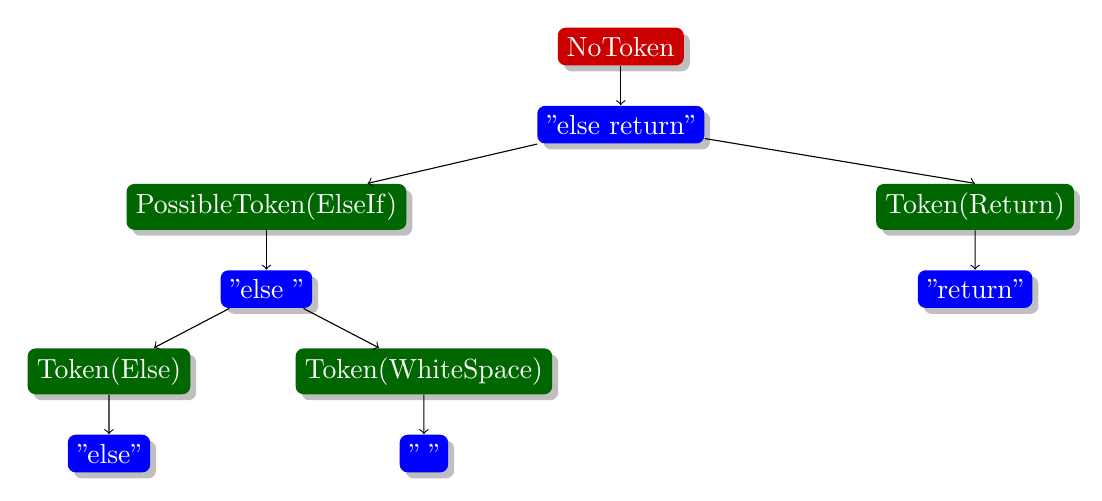
\begin{tikzpicture}[
    error/.style={rectangle, draw=none, rounded corners=1mm, fill=black!20!red, drop shadow,
        text centered, anchor=north, text=white},
    fact/.style={rectangle, draw=none, rounded corners=1mm, fill=black!60!green, drop shadow,
        text centered, anchor=north, text=white},
    state/.style={rectangle, draw=none, rounded corners=1mm, fill=blue, drop shadow,
        text centered, anchor=north, text=white},
    leaf/.style={rectangle, draw=none, rounded corners=1mm, fill=blue, drop shadow,
        text centered, anchor=north, text=white},
    level distance=0.5cm, growth parent anchor=south
    ]
    \node (State00) [error] {NoToken} [->]
        child{ [sibling distance=9cm]
            node (State01) [state] {"else return"}
            child{
                node (Fact02) [fact] {PossibleToken(ElseIf)}
                child{ [sibling distance=4cm]
                    node (State02) [state] {"else "}
                    child{
                        node (Fact03) [fact] {Token(Else)}
                        child{
                            node (State03) [leaf] {"else"}
                        }
                    }
                    child{
                        node (Fact04) [fact] {Token(WhiteSpace)}
                        child{ [sibling distance=1.2cm]
                            node (State04) [leaf] {" "}
                        }
                    }
                }
            }
            child{ [sibling distance=4cm]
                node (Fact05) [fact] {Token(Return)}
                child{
                    node (State05) [leaf] {"return"}
                }
            }
        }
    ;
  \end{tikzpicture}
  \caption{Lexer thinks "else " is an "else if" pattern. 
  \label{fig1:elseif}}
\end{figure}
From here when the lexer has found that there are no tokens for this lexeme it will try to split the left child token.
\begin{center}
    split("else ") => ["else"," "]
\end{center} 
Now the lexer has a pair of two lexems that represent valid tokens. The lexer knows that combinding these two lexems in the pair returns in a NoToken result. So The only thing to do is to try to combine the right token in the pair with the right child token and let the token to the left in the pair stand alone. 
\begin{figure}[!h]
  \centering
  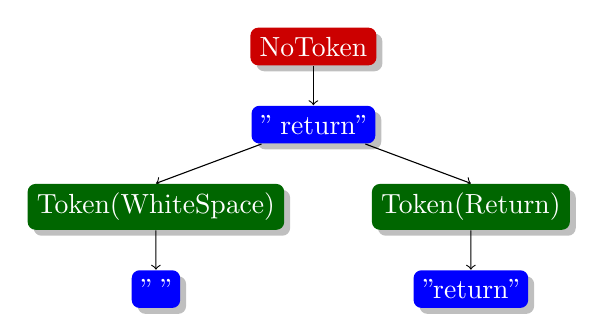
\begin{tikzpicture}[
    error/.style={rectangle, draw=none, rounded corners=1mm, fill=black!20!red, drop shadow,
        text centered, anchor=north, text=white},
    fact/.style={rectangle, draw=none, rounded corners=1mm, fill=black!60!green, drop shadow,
        text centered, anchor=north, text=white},
    state/.style={rectangle, draw=none, rounded corners=1mm, fill=blue, drop shadow,
        text centered, anchor=north, text=white},
    leaf/.style={rectangle, draw=none, rounded corners=1mm, fill=blue, drop shadow,
        text centered, anchor=north, text=white},
    level distance=0.5cm, growth parent anchor=south
    ]
    \node (State00) [error] {NoToken} [->]
        child{ [sibling distance=4cm]
            node (State01) [state] {" return"}
            child{ [sibling distance=4cm]
                node (State02) [fact] {Token(WhiteSpace)}
                child{
                    node (Fact02) [leaf] {" "}
                }
            }
            child{ [sibling distance=4cm]
                node (Fact03) [fact] {Token(Return)}
                child{
                    node (State03) [leaf] {"return"}
                }
            }
        }
    ;
  \end{tikzpicture}
  \caption{Lexer tries to combine an white space with a return statement
  \label{fig4:elseif}}
\end{figure}
This also return a NoToken. So the same thing will be done again. The lexer tries to split the left child before NoToken was given. In this case the whitespace. 
\begin{center}
split(" ") => []
\end{center}
But becouse the whitespace is of the lowest form and is not build up by smaller tokens the resulting list from the split function will be empty. Now the lexer knows that this token must be by it self. The "return" is the last lexeme in this example code so the lexer can't combine it futher. Thus the lexer has found the resulting sequence of tokens:
\begin{center}
    [(Token(Else), "else"), (Token(WhiteSpace)," "), (Token(Return), "return")]
\end{center} 
\end{example}

\subsection{Dont know what to call this!}
When the code is divided the lexer doesn't know if the string (or character) it
lexes is the first, last or is somewhere in the middle of a token. Instead of
checking what type of token the string will be (if it were to begin from the
starting state) it saves all the possible state transitions for that string.

In the examples that follow below state 0 is considered the starting state and
state $1-6$ are considered accepting.
\begin{example}[Transition map for a token]\label{transMap}
A hypothetical transition map for the char 'i'.
\begin{center}$\begin{array}{cc}
\multicolumn{2}{c}{'i'}\\
in & out\\
0 & 1\\
1 & 1\\
8 & 7\\
\end{array}$\\
\end{center}
\end{example}
In the base case the lexer will map all the transitions for all individual
characters in the code and construct partial tokens of them. The conquer step
will then combine two of these at a time by checking which possible outgoing
states from the first token can be matched with incoming states from the second
token. If there are such pairs of outgoing states with incomming states, then a
new partial token is created.
\begin{example}[Combining two tokens]\label{combTok}
'if' can be an ident (state 1) or part of 'else if' (state 5).
\begin{center}$\begin{array}{cc}
\multicolumn{2}{c}{'i'}\\
in & out\\
\textcolor{brown}{0} & \textcolor{brown}{1}\\
1 & 1\\
\textcolor{blue}{8} & \textcolor{blue}{7}\\
\end{array}
`combineToken`
\begin{array}{cc}\multicolumn{2}{c}{'f'}\\
in & out\\
0 & 1\\
\textcolor{brown}{1} & \textcolor{brown}{1}\\
\textcolor{blue}{7} & \textcolor{blue}{5}\\
\end{array}
=
\begin{array}{cc}\multicolumn{2}{c}{'if'}\\
in & out\\
\textcolor{brown}{0} & \textcolor{brown}{1}\\
\textcolor{blue}{8} & \textcolor{blue}{5}\\
\end{array}$\\
\end{center}
\end{example}
If there are no pairs of outgoing states which match the incomming states the
lexer will try to combine the first token with as much of the second token as
possible. In this case there will be a remainder of the second token, The lexer
can now be sure that the begining of the remainder is the begining of a token
and that the merged part is the end of the token before.
Since the lexer knows the remainder is the begining of a token it strips all
transitions but the one that has incomming state as starting state. Since the
start token is the end of a Token it strips all but the transitions ending in an
accepting state.
\begin{example}[Combining a token a part of the second token]\label{combSplit}
'ie' ends in the accepting state for ident (1) and '\_' starts in the
starting state.
\begin{center}
$\begin{array}{cc}\multicolumn{2}{c}{'e\_'}\\
in & out\\
\textcolor{brown}{10} & \textcolor{brown}{8}\\
\end{array}
=
\begin{array}{cc}\multicolumn{2}{c}{'e'}\\
in & out\\
0 & 11\\
\textcolor{blue}{1} & \textcolor{blue}{1}\\
6 & 1\\
\textcolor{brown}{10} & \textcolor{brown}{9}\\
\end{array}
`combineToken`
\begin{array}{cc}\multicolumn{2}{c}{'\_'}\\
in & out\\
0 & 2\\
2 & 2\\
\textcolor{brown}{9} & \textcolor{brown}{8}\\
\end{array}
$\\
$\begin{array}{cc}
\multicolumn{2}{c}{'i'}\\
in & out\\
\textcolor{blue}{0} & \textcolor{blue}{1}\\
\textcolor{blue}{1} & \textcolor{blue}{1}\\
8 & 7\\
\end{array}
`combineToken`
\begin{array}{cc}\multicolumn{2}{c}{'e\_'}\\
in & out\\
10 & 8\\
\end{array}
=
\begin{array}{cc}\multicolumn{2}{c}{'ie'}\\
in & out\\
\textcolor{blue}{0} & \textcolor{blue}{1}\\
\textcolor{blue}{1} & \textcolor{blue}{1}\\
\end{array} ++ 
\begin{array}{cc}\multicolumn{2}{c}{'\_'}\\
in & out\\
0 & 2\\
\end{array}$\\
\end{center}
\end{example}
\# Perhaps remove this part\\
However the remainder may not have the start state as a possible incomming state.
In this case the lexer tries to find the largest possible token (that has the
starting state as incomming state) and tries to construct a token of the rest of
the remainder, repeating this procedure until the entire remainder has been
split into acceptable tokens. All the tokens accept the one that is on the very
end of the sequence will have all but their accepting states stripped. This case
does occur quite frequently since most languages has comments and strings which
can contain anything.
\begin{example}[Handling the remainder]\label{remToken}
'\_' starts in the starting states and ends in an accepting state and 'e' starts
in the starting state, it doesn't have to end in an accepting state.
\begin{center}
$\begin{array}{cc}\multicolumn{2}{c}{'\_i'}\\
in & out\\
\textcolor{brown}{9} & \textcolor{brown}{7}\\
\end{array}
=
\begin{array}{cc}\multicolumn{2}{c}{'\_'}\\
in & out\\
0 & 2\\
2 & 2\\
\textcolor{brown}{9} & \textcolor{brown}{8}\\
\end{array}
`combineToken`
\begin{array}{cc}
\multicolumn{2}{c}{'i'}\\
in & out\\
0 & 1\\
1 & 1\\
\textcolor{brown}{8} & \textcolor{brown}{7}\\
\end{array}$\\
$checkRemainder \left(\begin{array}{cc}\multicolumn{2}{c}{'\_i'}\\
in & out\\
9 & 7\\
\end{array} \right)
=
\begin{array}{cc}\multicolumn{2}{c}{'\_'}\\
in & out\\
0 & 2\\
\end{array} ++
\begin{array}{cc}\multicolumn{2}{c}{'i'}\\
in & out\\
0 & 1\\
\end{array}$\\
\end{center}
\end{example}
When all partial tokens has been combined in this way the resulting sequence of
tokens represents the the code the lexer was run on.


\chapter{Conclusion and Future Work}
As mentioned in the result chapter the incremental lexer was both robust and
precise. This means that without considering the time and space effiency an
incremental lexer will produce the same result as a sequential lexer with the
difference being how lexical errors are handled. The incremental lexer is
efficient in the sense that updates are done in $\Theta \log(n)$ time. However
when a tree is built up from scratch the incremental lexer takes
$\Theta n\log(n)$ time compared to the sequential lexer that takes $\Theta n$
time.

\section{Conclusions}
Incremental lexers is not suited to be used in a stand alone lexer since a
sequential lexer is more effiecent then an incremental lexer when an entire text
is being lexed. If a development environment that uses an incremental lexer was
used, the stand alone lexer can be omitted since the tokens are already
generated, saving one step in the compilation process.

It is however suited in an environment where updates are likely to happen, for
example to give lexical feedback in a text editor where each key stroke would be
an update. Insertion of a character in the text will be faster with an
incremental lexer compared to a sequential lexer since the lexical analysis does
not need to be done on the entire text. This means that the lexer could be run
in real time without a user noticing it. The result from an incremental lexer
can be passed to an incremental parser, giving parsing feedback to the user
instead. However, loading times when opening files will be longer if the tree
containing the tokens are not stored.

The space requirements for the incremental lexer grows with the tree. There is
information for the entire text in all levels of the tree and each level has
information for all possible in states. The space of a tree grows with
$\Theta mn\log(n)$, where $m$ is the number of states in the DFA. This means
that the memory usage will be big for large files and complex languages.

\section{Future Work}
To solve the problem with the space requirements for this implementation an
implementation using sequence of characters could be used instead. That is,
instead of using a character as the base case, a sequence of characters is used
which is sequentially lexed, an example of a sequence is one line of code. This
would shrink the tree from $\log(n)$ to $\log(n/x)$ where x is the mean length
of a line. Since lines in the code is roughly of the same length there will be
no impact on the worst case scenario time, for instance lexing 10 characters
always takes the same amount of time. Since the lines in general are short
updating a line will not take long time.

Another solution which could be used is to limit how big a tree can be. When
that text is bigger then what fits in a tree, the tree is split into two trees.
This will result in smaller trees at the expense of run time since the
combination of the trees needs to be calculated on the fly.

In general a lot of in states will have the same sequence of tokens. The
implementation suggested by this report will store all such sequences
separately. An improvement would be if somehow the sequences of tokens that are
identical could be stored in a separate table and the in state in the transition
map points to the corresponding sequence for that in state. This would not
improve the space complexity, but he practical space needed would shrink.


\newpage
\clearpage

% Nocite references

\bibliography{references} % references.bib
\addcontentsline{toc}{chapter}{\numberline{} Bibliography} % For pdf
\setspecialhdr

\newpage

% Appendices
\appendix
\setdefaulthdr
%\input{include/appendix1}
\end{document}
